The simulator in TVB resembles popular neural network simulators in 
many fundamental ways, both mathematically and in terms of informatics 
structures, however we have found it necessary to introduce auxiliary
concepts particularly useful in the modeling of large scale brain 
networks.

% need to cite Andreas' work and 
\note[psl] {just being picky... In other works of large scale brain modeling, the network structure is described before the node dynamics.} 


\subsection{Node dynamics}

    In TVB, nodes are not considered to be abstract neurons nor necessarily
    small groups thereof, but rather large populations of neurons. Concretely,
    the main assumption of the neural mass modeling approach in TVB is that
    large pools of neurons on the millimeter scale are strongly approximated
    by population level equations describing the major statistical modes of
    neural dynamics \cite{Freeman_1975book}. Often, averaging techniques are
    employed, though techniques retaining several modes have been developed
    \cite{Stefanescu_2008, Stefanescu_2011}. Such an approach is certainly not
    new; one of the early examples of this approach consist of the well known
    Wilson-Cowan equations \cite{Wilson_1973}. Nevertheless, there are
    important differences in the the assumptions and goals from modeling of
    individual neurons, where the goal may be to reproduce correct spike
    timing or predict the effect of  a specific neurotransmitter. A second
    difference lies in coupling: chemical coupling is often assumed to be
    pulsatile, or discrete, between neurons, whereas it is considered
    continuous. Typically the goal of neural mass modeling is to study the
    dynamics that emerge from the interaction of two or more neural masses and
    the network conditions required for stability of a particular
    spatiotemporal pattern. In the following, we shall  briefly discuss some
    of the models available in TVB.

    As we have noted, many neural mass models have been developed. One of
    the more prominent examples in the systems neuroscience literature is 
    that the Jansen-Rit model of rhythms and evoked responses arising from
    coupled cortical column \cite{Zetterberg_1978, Jansen_1995, Spiegler_2010}. 
    \note[mw]{Continue description}.
    \note[psl]{maybe see David et al, 2004 for better description of local connectivity in the Jansen and Rit model}
    Advantages of the Jansen-Rit model stem from the connection made
    between empirical studies of neural tissue and the model's parameters, 
    making it easier in certain cases to make concrete predictions about
    the relation between a dynamical regime and its neurobiological 
    mechanism. However, because the form of the model used often employs
    at least six dimensions, it is not always clear how to analyze or
    visualize. Lastly, the model requires frequent computation of exponentials,
    requiring considerable computational time. 

    For these reasons, it is often desirable to have a simpler mathematical 
    model, which may be reproduce the same qualitative phenomena as other 
    models, implemented with fewer and simpler equations. Such is the motivation
    for the generic two-dimensional oscillator model provided by TVB. 
    \note[mw]{Continue}. This model produces oscillations, damped, spike-like or 
    sinusoidal activations, while requiring less time to solve.

    However, the modeler's goals may not lead to either the Jansen-Rit
    \cite{Jansen_1995, David_2003, David_2004} or generic 2D oscillator
    \cite{FitzHugh_1961, Nagumo_1962}, and several other mass models are
    provided by TVB: the previously mentioned Wilson-Cowan description of
    functional dynamics of neural tissue \cite{Wilson_1972}, the Kuramoto
    model describing synchronization \cite{Kuramoto_1975, Cabral_2011}, two
    and three dimensional mode-level models describing populations with
    excitability distributions \cite{Stefanescu_2011, Stefanescu_2008}, a
    reduction of the Wong and Wang model \cite{Wong_2006} as presented in
    \cite{Deco_2013} and a lumped version of Liley's model \cite{Liley_1999,
    Steyn-Ross_1999} model are among the available models in TVB.

    Again, should any of these be insufficient, a new model can be implemented
    with minimal effort by subclassing a base \texttt{Model} class and
    providing a  \texttt{dfun} method to compute the right hand sides of the
    differential  equations. Please refer to the \url{https://github.com/the-
    virtual-brain/scientific_library/tree/trunk/contrib/simulator/models} for
    examples. In here, models found in the work of \cite{Larter_1999,
    Breakspear_2003, Morris_1981, Hindmarsh_1984, Brunel_2001} have been implemented.

    

\subsection{Network structure}

    The network of neural masses in TVB simulations directly follows from  a
    pair of geometrical constraints on cortical dynamics. The first is the
    large-scale white matter fibers that form a non-local and heterogeneous
    (translation variant) connectivity, either measured by anatomical tracing
    (CoCoMac\ref{CoCoMac}) or diffusion-weighted imaging \cite{Hagmann_2008,
    Honey_2009, Bastiani_2012}. The second is that of horizontal projections
    along the surface, which are modeled through a translation invariant
    \note[sk]{Not technically true, using singular parameters will produce
    this but that's only a limited subset of the capability, spatially
    inhomogeneous parameters are supported -- thus being more general than the
    restricted case of translational invariance} connectivity kernel,
    approximating a neural field.

    \subsubsection{Large-scale connectivity}

    The large-scale region level connectivity at the scale of centimeters,
    resembles more a traditional neural network than a neural field in that
    neural space is discrete,  each node corresponding to a neuroanatomical
    region of interest, such as V1, etc. It is at this level that inter-
    regional time delays play a large role.
    \note[psl]{In the case of neural field modelling, time delays at the local level would also play a role} 

    It is often seen in the literature that the inter-node coupling functions
    \textit{are} part of the node model itself. In TVB, we have instead 
    chosen to factor such models into the intrinsic neural mass dynamics, where each 
    neural mass's equations specify how connectivity contributes to the
    node dynamics, and the coupling function, which specifies how the activity
    from each region is mapped through the connectivity matrix. Common coupling 
    functions are provided such as the linear, difference and periodic functions
    often used in the literature.

    \subsubsection{Local connectivity}

    The local connectivity of the cortex at the scale of millimeters provides
    a continuous 2D surface along horizontal projections connect 
    cortical columns. Such a structure has previously been modeled by
    neural fields \cite{Amari_1977, Jirsa_1997, Liley_1999}. In TVB, a cortical mesh, 
    as obtained from structural MRI data and simplified, provides a spatial 
    discretization on which neural masses are placed and connected with a
    local connectivity kernel, itself only a function of the geodesic distance
    between the two masses, and this is considered to provide an
    approximation of a neural field, depending on the properties
    of the mesh and the imaging modalities that sample the activity simulated
    on the mesh \cite{Spiegler_2013}. 
    \note[sk]{The implementation of the local connectivity kernel is such
    that is can be re-purposed as a discrete Laplace-Beltrami operator,
    allowing for the implementation of true neural-field models that 
    use a second-order spatial derivative as their explicit spatial term.}

    TVB currently provides several connectivity kernels, among others, 
    the Laplacian and Gaussian kernels. Once a cortical surface mesh 
    and connectivity kernel and its parameters are chosen, the geodesic
    distance (i.e. the distance along the cortical surface) is evaluated
    between all neural masses \cite{Mitchell1987}, and a cutoff is chosen
    past which the kernel falls to 0. This results in a sparse matrix that 
    is used during integration to implement the approximate neural field. 
    \note[psl]{The Laplacian kernel is not implemented yet.}

\subsection{Integration of stochastic delay differential equations}

    In order to obtain numerical approximations of the large-scale brain network model 
    described above, \TVB provides several numerical integration methods. For
    deterministic simulations, the well-known Euler, 
    Heun and Runge-Kutta 4th order 
    \note[sk]{Probably best not to mention rk4 as it's only available 
    for isolated model integration, ie no networked delays...}
    algorithms are available. For stochastic
    simulations, stochastic Euler and Heun integrators are available, 
    following recent literature on numerical solutions to stochastic
    differential equations \cite{Kloeden_1995,Mannella_2002,Mannella_1989}.

    While the literature on numerical treatment of delayed or 
    stochastic systems exists, it is less well known how to treat 
    the presence of both. For the moment, the methods implemented by TVB
    treat stochastic integration separately from delays. 
    This separation conincides with a modeling assumption that in
    TVB the dynamical phenomena to be studied are largely determined
    by the interaction of the network structure and neural mass dynamics, 
    and that stochastic fluctuations do not fundamentally reorganize the
    solutions of the system \cite{Ghosh_2008,Deco_2009,Deco_2011,Deco_Senden_2012}.

    Due to such a separation, the implementation of delays in the
    regional coupling is performed outside the integration step,
    by indexing a circular buffer containing the recent simulation 
    history, and providing a matrix of delayed state data to the 
    network of neural masses. While the number of pairwise
    connections rises with $N^2$, only one buffer per region 
    is stored with a length corresponding to the longest projection
    from that region.
    \note[sk]{Unless something has changed, I'm fairly sure the 
    length of the history is set based on the longest projection
    of the whole network and not specific per region...}

\subsection{Forward solutions}

    A primary goal of TVB is not only to model neural activity itself
    but just as importantly the imaging modalities common in human 
    neurosciences, using so-called forward solutions, which allow for
    the projection of neural activity into sensor space. To account
    parsimoniously for other ways in which simulated data might be saved, 
    such as simple temporal averaging, we refer to each of these simply as 
    \textit{Monitors}, which take as input neural activity and 
    output a particular projection thereof. In most cases, this 
    takes the discrete-time form of

    \[ \hat{y}[j, t] = \sum_{i=1, \tau=1}^{N_W, N_k} W[j, i] K[\tau] y[i, t-\tau] \]

    \noindent where $y[i, t]$ is the amplitude of the $i^{th}$ neural mass at time
    $t$, $K[\tau]$ is a temporal kernel, and $W[j, i]$ is a spatial kernel,
    usually projecting the state variable of interest of the $i^{th}$ 
    neural mass to the $j^{th}$ sensor. 

    Where necessary for computational reasons, monitors employ more than 
    one internal buffer. The fMRI monitor is one 
    example: given a typical sampling frequency of simulation may be upward of 
    64 kHz, and the haemodynamic response function may last several seconds, 
    requiring many gigabytes of memory for the fMRI monitor alone. Given that 
    the time-scale of simulation and fMRI differ by several orders of magnitude, 
    the subsequent averaging and downsampling is entirely justified. 

    In the cases of the EEG and MEG monitors, $K$ implements a simple
    temporal average, and $W$ consists of a so-called lead-field matrix as typically
    derived from a combination of structural imaging data of the patient 
    and the locations and orientations of the neural sources and the locations
    and orientions of the EEG electrodes and MEG gradiometers and magnetometers. 
    As the development and implementation of such lead-fields is well developed
    elsewhere \cite{Jirsa_2002,Nolte2003,Gramfort_2010}, TVB provides access
    to the well-known OpenMEEG package, however, the user is free to provide 
    his or her own.

\subsection{Native code generation for C \& GPU}

    Several of the core components (integrators, mass models, coupling
    functions) have targeted towards a C source code backend, which has
    allowed for the compilation of simulations to native code loaded 
    either as a shared library accessed via the \texttt{ctypes} modules
    or as CUDA kernels accessed via the PyCUDA \cite{PyCUDA}.
    While such an approach may provide speed ups, they depend on the
    presence of a C compiler and, in the case of GPU, the CUDA toolkit and
    a compatible graphics card, and in the future, prepackaged versions of TVB
    will include precompiled objects for most kinds of simulations. 

    The approach used in compiling a simulation to native code takes advantage
    of the fact that CUDA is quite similar to C, and thus a generic template
    abstracts much of the boilerplate between the two. For each part of the 
    simulator, a generic function is customized with a class specific kernel;
    for example, in the case of a neural mass model, we have in the Python class

    \begin{lstlisting}
    class Generic2dOscillator(Model):
        tau = FloatArray(...)
        # etc.

        device_info = model_device_info(
        pars=[tau, a, b, c, d, I],
        kernel="""
        float tau  = P(0)
            , a    = P(1) ; // etc

        // state variables
            , v    = X(0)
            , w    = X(1)

        // aux variables
            , c_0  = I(0)   ;

        // derivatives
        DX(0) = d * 
        (tau * (w - v*v*v + 3.0*v*v + I + c_0));
        DX(1) = d * 
        ((a + b*v + c*v*v - w) / tau);
        """
        )
    \end{lstlisting}

    \noindent where the device\_info attribute is used to specify how the
    class's mathematical description fits into the general model function:

    \begin{lstlisting}
    /* wrapper for model specific code computing RHSs of diff-eqs */
    __device__
    void model_dfun(
      float * _dx, float *_x, float *mmpr, float *input)
    {
    #define X(i) _x[n_thr*i]
    #define DX(i) _dx[n_thr*i]
    #define P(i) mmpr[n_thr*i]
    #define I(i) input[i]

        // begin model code
        \$model_dfun
        // end model specific code

    #undef X
    #undef DX
    #undef P
    #undef I
    \end{lstlisting}

    \noindent where the C preprocessor defines allow the model specific
    kernel to easily reference the correct parts of the multidimensional 
    per-thread arrays (in the case of the GPU). 

     \begin{figure}
        {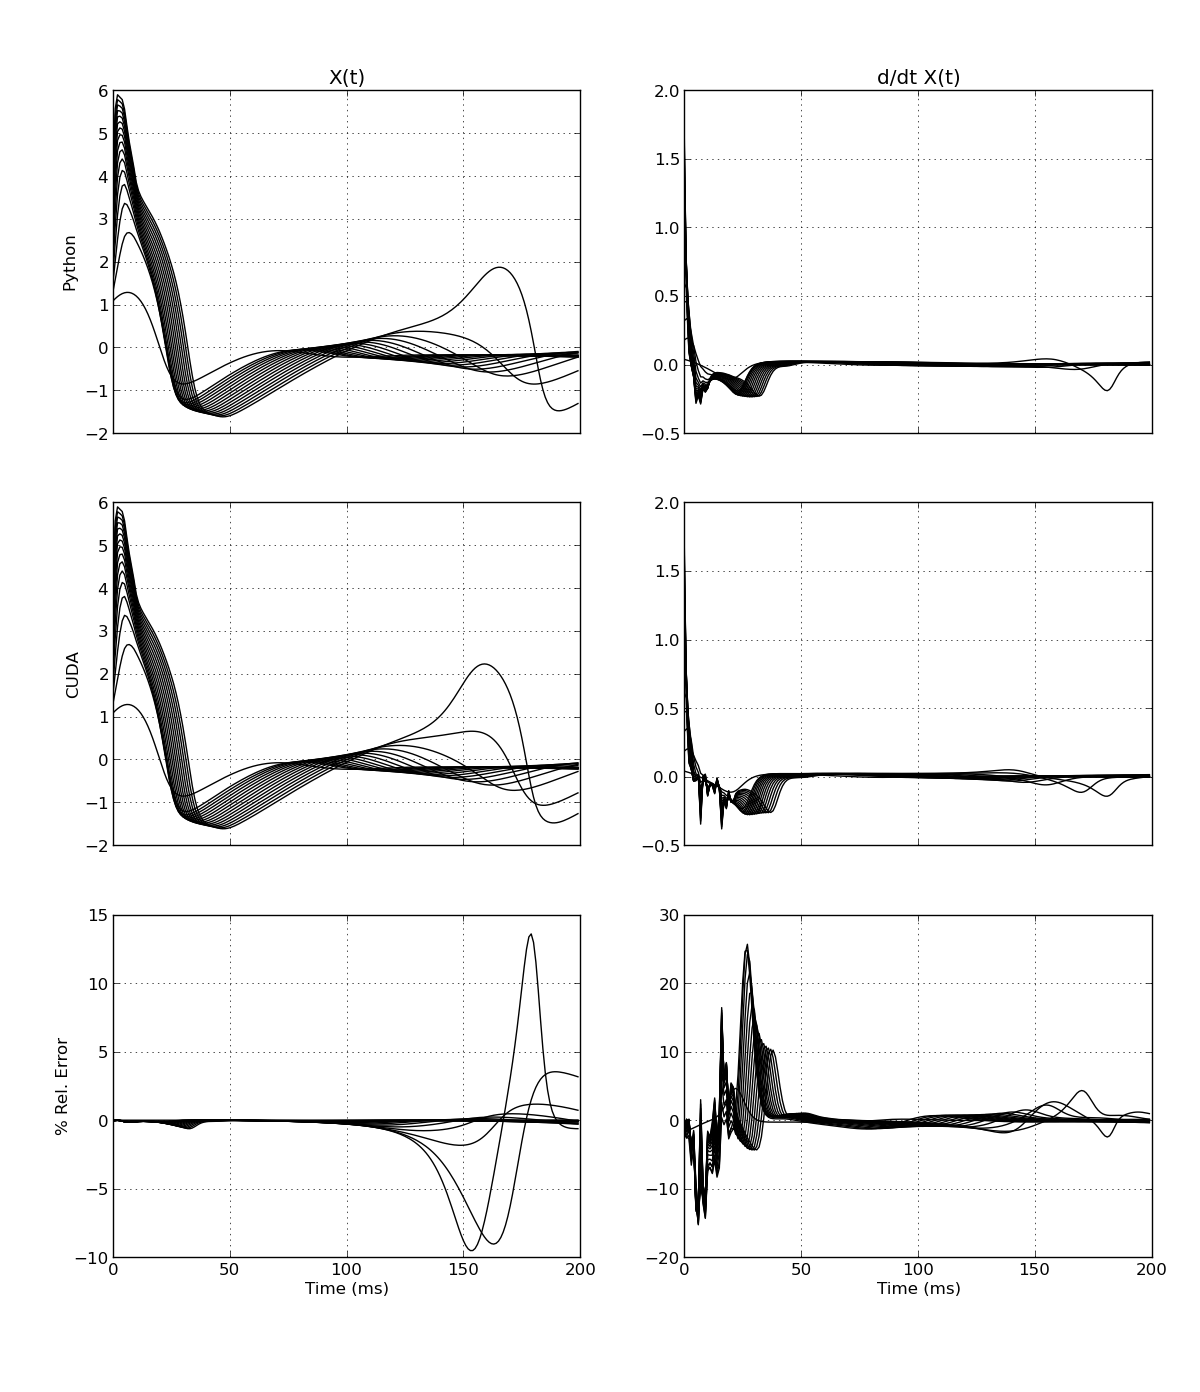
\includegraphics[width=0.48\textwidth]{images/gpu_dxdt.png}}
        \caption{
        Right A typical parameter space exploration, 32 x 32 grid of
        coupling strength (y-axis) v. neural excitability (x-axis).
        This grid of simulations was run on both TVB's Python/NumPy
        implementation and the new GPU backend for 200 ms simulation
        time with otherwise default parameters. The former took ~2
        hours and the latter ~ 1 min. Left Quantitative comparison of
        solutions and instantaneous derivatives is shown for an even
        sampling of the parameter space across k where a = -2, because
        this slice showed the most error on the GPU.    
        }
        \label{fig:gpu_dxdt}
    \end{figure}

     \begin{figure}
        {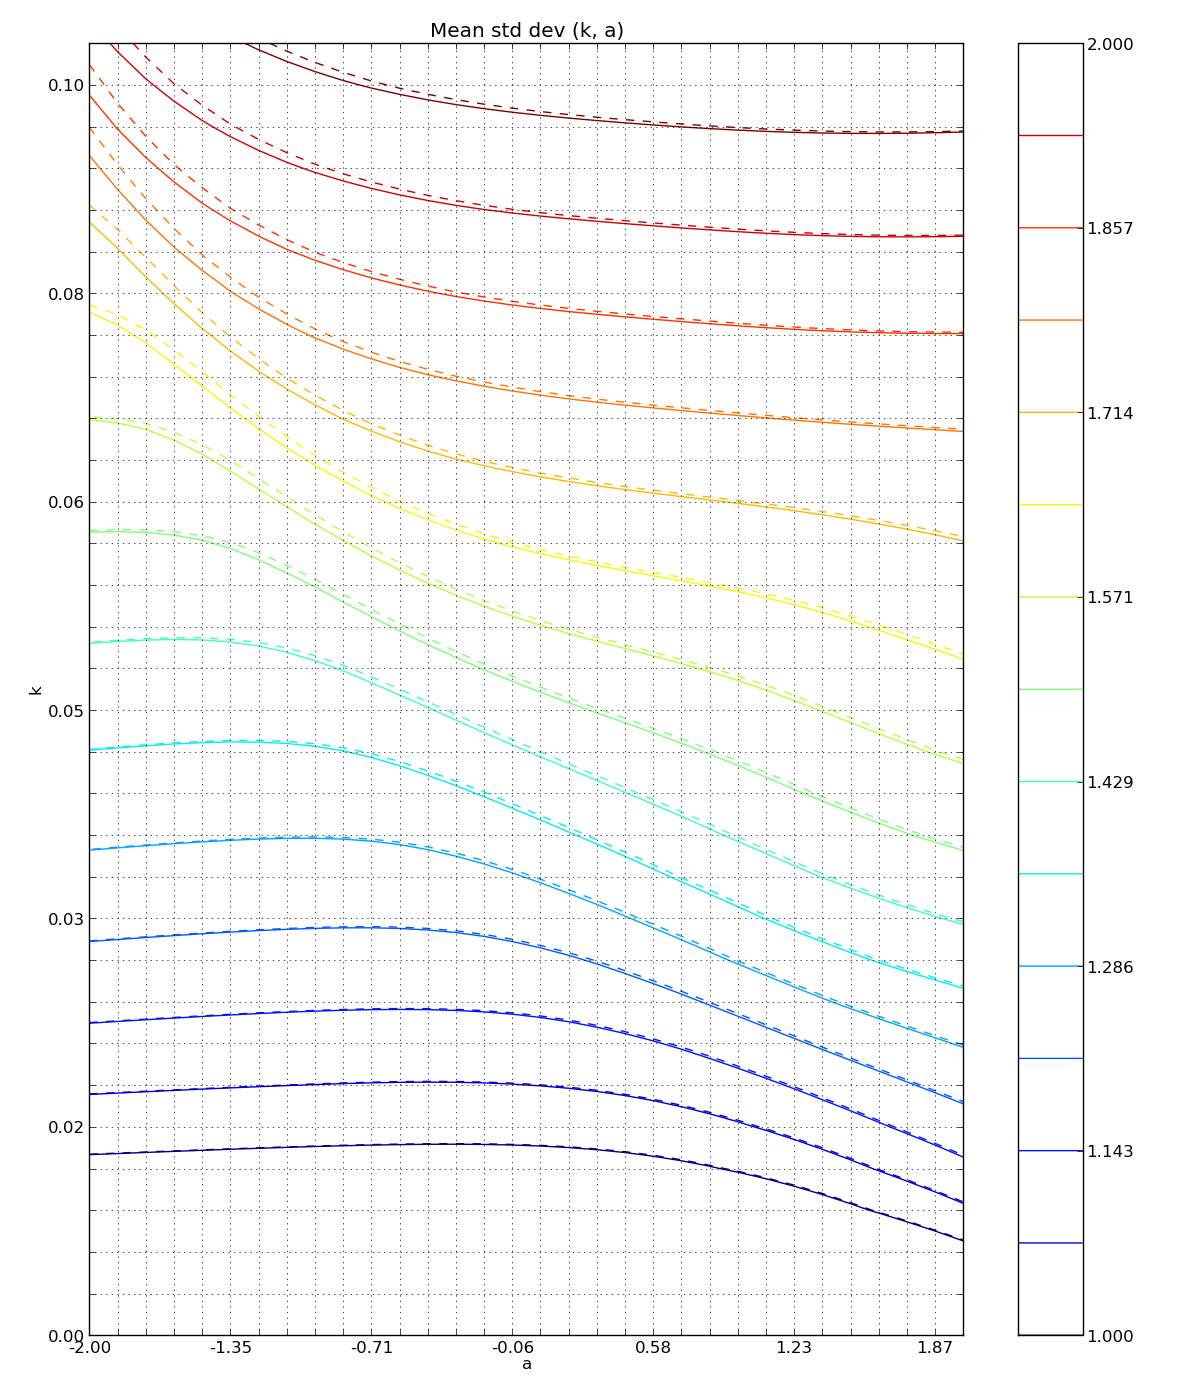
\includegraphics[width=0.48\textwidth]{images/gpu_pse.png}}
        \caption{}
        \label{fig:gpu_pse}
    \end{figure}

    \note[sk]{One figure or two, re captions}

    \note[sk]{Specify hardware (GPU/CPU) and whether Numpy is mkl-linked, to 
        provide a more solid foundation for timing comparisons...}

    \note[sk]{It would be interesting to see a longer run (say a few seconds)
        to show if/how-quickly the error grows...}

    As can be seen in the listing \note[sk]{can listings be numbered and labelled...}, the calculations
    in native code are performed with 32-bit floating point numbers, and it
    is reasonable to ask if this is numerically accurate. In Fig 
    \ref{fig:gpu_pse}, we present a parameter space exploration performed with
    both the pure Python NumPy simulator and the GPU simulator, showing the 
    isocontours of average standard deviation in the parameter space. Some
    deviation can be identified visually in parts of the parameter space, and
    in in Fig \ref{fig:gpu_dxdt}, we show in more detail time series of 
    the Python and GPU solutions.

     \begin{figure}
        {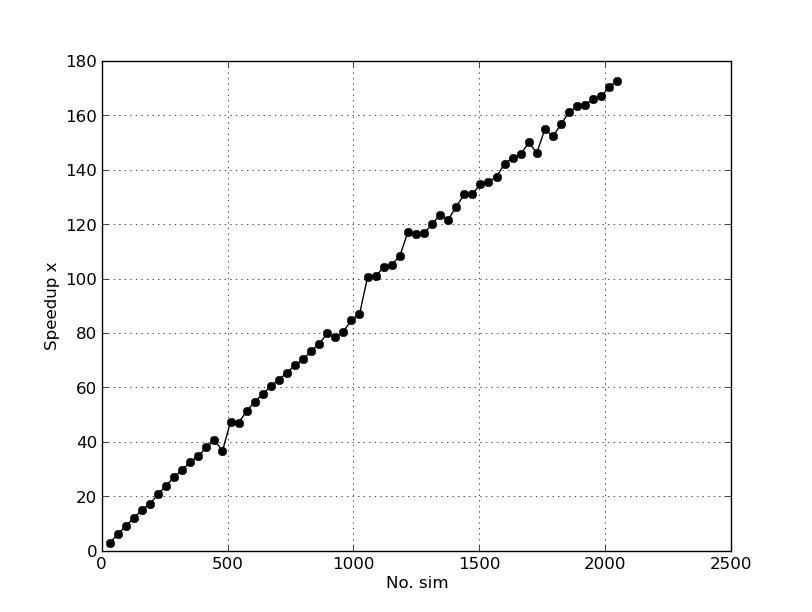
\includegraphics[width=0.48\textwidth]{images/gpu_acceleration.png}}
        \caption{}
        \label{fig:gpu_acceleration}
    \end{figure}

    This approach allows significant acceleration of parameter sweeps in the
    case of the GPU by taking
    advantage of the fact that in many cases, only numerical values vary
    between different threads and not memory access patterns. Where one of the
    dimensions of a parameter sweep implies changing memory access patterns, 
    for example conduction speed, it is advantageous to reorder the parameters,
    so that such memory varying parameters only change between grids of GPU
    threads and not within.

    In Fig \ref{fig:gpu_acceleration}, we plot the speedup brought by the GPU
    over the Python NumPy simulator as a function of the number of simulations 
    performed simulataneously on the GPU.


\subsection{Other simulators compared to TVB}

    Brian should be a particular focus in this section, as it may
    be one of the closest. 

    - several spiking models in the literature use the notain of a reset
        condition and potential, for which Brian provides explicit
        functionality. TVB does not because typically the deterministic
        dynamics of neural mass models are continuous.
